\section{Sprint 1: Core Administrative APIs}

\subsection{Objectives}
Sprint 1 focused on building the foundational administrative APIs that define the company’s structure and workforce.  
The main goal was to implement full CRUD operations for Employees, Branches, Departments, and Designations, ensuring all entities could be created, updated, deleted, and retrieved securely.  
Bulk operations such as Import/Export for Employees were also introduced.

\subsection{Tasks Completed}
\begin{itemize}
    \item Implemented CRUD APIs for the following entities:
    \begin{itemize}
        \item Employees (with Import \& Export functionality).
        \item Branches.
        \item Departments.
        \item Designations.
    \end{itemize}
    \item Secured all endpoints with JWT authentication middleware.
    \item Documented endpoints and tested responses in Postman.
    \item Updated database schema to support relations (Employees linked to Departments, Branches, and Designations).
\end{itemize}

\subsection{Outputs}
By the end of Sprint 1, the following deliverables were achieved:
\begin{itemize}
    \item Functional APIs for organizational entities.
    \item Secure JWT-protected CRUD endpoints.
    \item Initial dataset for Employees, Branches, Departments, and Designations.
    \item Verified API responses through Postman.
\end{itemize}

% --------------------------------------------------------
% USE CASE DIAGRAM
% --------------------------------------------------------
\subsection{Administrative Use Case Diagram}
\begin{figure}[H]
    \centering
    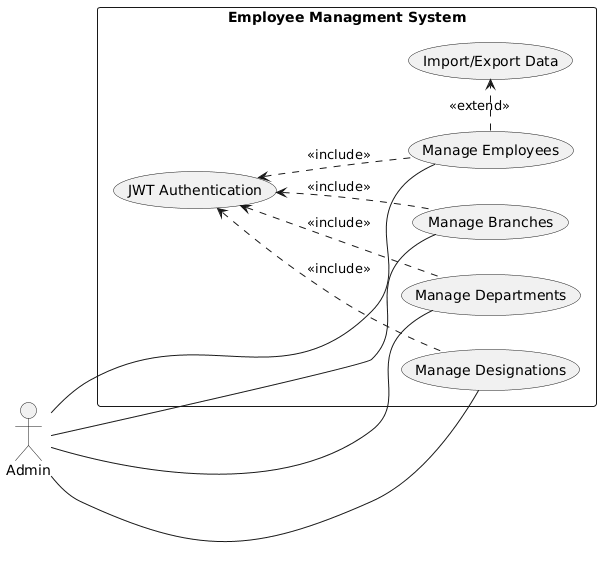
\includegraphics[width=0.85\textwidth]{chapters/chapter 3/sprint1_figures/use_case_Employee-managment.png}
    \caption{Use Case Diagram for Administrative APIs (Employees, Branches, Departments, Designations)}
    \label{fig:sprint1_usecase}
\end{figure}

% --------------------------------------------------------
% USE CASE SCENARIO TABLE
% --------------------------------------------------------
\subsection{Use Case Scenario: Create Employee}
\begin{longtable}{|p{3cm}|p{11cm}|}
\hline
\textbf{Use Case} & Create Employee Record \\
\hline
\textbf{Actor} & Admin \\
\hline
\textbf{Preconditions} & 
\begin{itemize}
    \item Admin is authenticated with a valid JWT token.
    \item The system has at least one Branch, Department, and Designation defined.
\end{itemize} \\
\hline
\textbf{Main Flow} &
\begin{enumerate}
    \item Admin selects ``Add Employee'' option in the application.
    \item System sends a \texttt{POST /employees} request with employee details (name, email, salary, branch\_id, department\_id, designation\_id).
    \item API validates request payload.
    \item API stores the new employee in the database.
    \item System returns a \texttt{201 Created} response with employee details.
\end{enumerate} \\
\hline
\textbf{Alternative Flows} &
\begin{itemize}
    \item \textbf{A1: Missing/Invalid Token:} System returns \texttt{401 Unauthorized}.
    \item \textbf{A2: Invalid Data:} System returns \texttt{422 Unprocessable Entity} with validation errors.
    \item \textbf{A3: Foreign Key Missing:} If Branch/Department/Designation ID does not exist, system returns \texttt{404 Not Found}.
\end{itemize} \\
\hline
\textbf{Postconditions} & 
\begin{itemize}
    \item A new employee record is created and stored in the database.
    \item Employee is now linked to Branch, Department, and Designation entities.
\end{itemize} \\
\hline
\caption{Use Case Scenario: Create Employee (Sprint 1)}
\label{tab:usecase_create_employee}
\end{longtable}

% --------------------------------------------------------
% SEQUENCE DIAGRAM
% --------------------------------------------------------
\subsection{Sequence Diagram: Create Employee}
\begin{figure}[H]
    \centering
    \includegraphics[width=0.9\textwidth]{}
    \caption{Sequence Diagram for Create Employee API}
    \label{fig:sprint1_sequence}
\end{figure}

% --------------------------------------------------------
% CLASS DIAGRAM
% --------------------------------------------------------
\subsection{Class Diagram: Administrative Entities}
\begin{figure}[H]
    \centering
    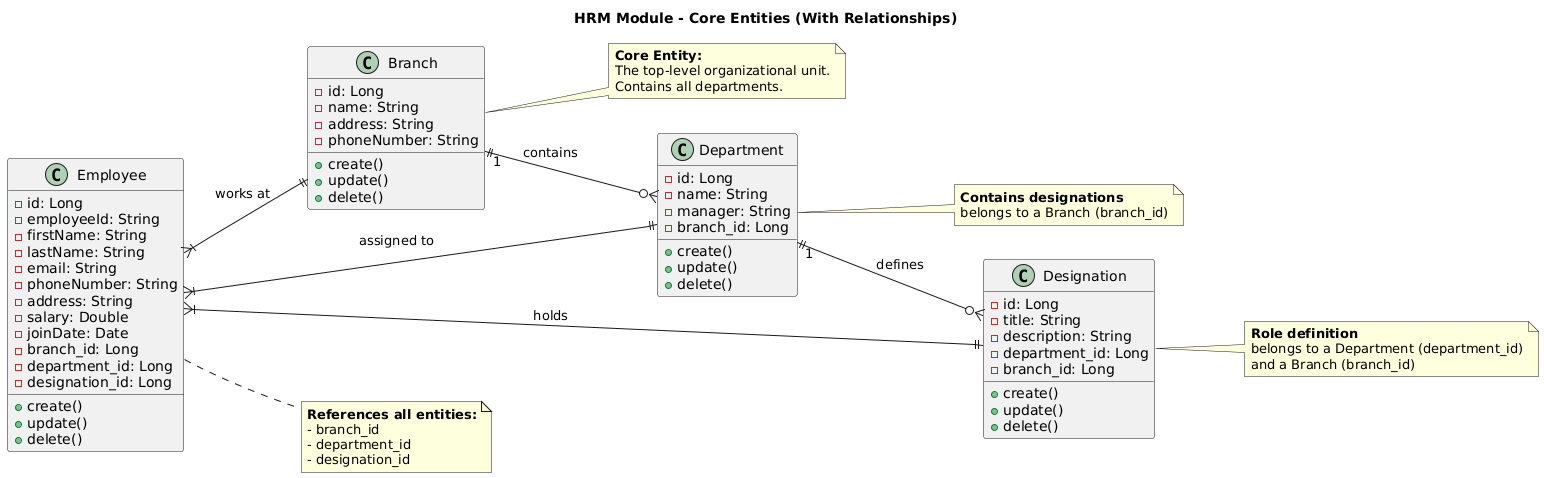
\includegraphics[width=0.85\textwidth]{chapters/chapter 3/sprint1_figures/class_diagram_s1.png}
    \caption{Class Diagram for Employees, Branches, Departments, and Designations}
    \label{fig:sprint1_class}
\end{figure}

% --------------------------------------------------------
% API TESTING WITH POSTMAN
% --------------------------------------------------------
\subsection{API Testing with Postman}
The CRUD endpoints were tested using Postman to ensure correct functionality. Below are placeholders for screenshots:

\begin{figure}[H]
    \centering
    \includegraphics[width=0.8\textwidth]{chapters/chapter 3/sprint1Figures/postman_create_employee.png}
    \caption{Postman Test -- Create Employee API}
    \label{fig:postman_create_employee}
\end{figure}

\begin{figure}[H]
    \centering
    \includegraphics[width=0.8\textwidth]{chapters/chapter 3/sprint1Figures/postman_get_employees.png}
    \caption{Postman Test -- Get All Employees API}
    \label{fig:postman_get_employees}
\end{figure}

\begin{figure}[H]
    \centering
    \includegraphics[width=0.8\textwidth]{chapters/chapter 3/sprint1Figures/postman_update_employee.png}
    \caption{Postman Test -- Update Employee API}
    \label{fig:postman_update_employee}
\end{figure}

\begin{figure}[H]
    \centering
    \includegraphics[width=0.8\textwidth]{chapters/chapter 3/sprint1Figures/postman_delete_employee.png}
    \caption{Postman Test -- Delete Employee API}
    \label{fig:postman_delete_employee}
\end{figure}
